\documentclass{standalone}
\usepackage{tikz}
\usetikzlibrary{patterns, positioning}


\begin{document}
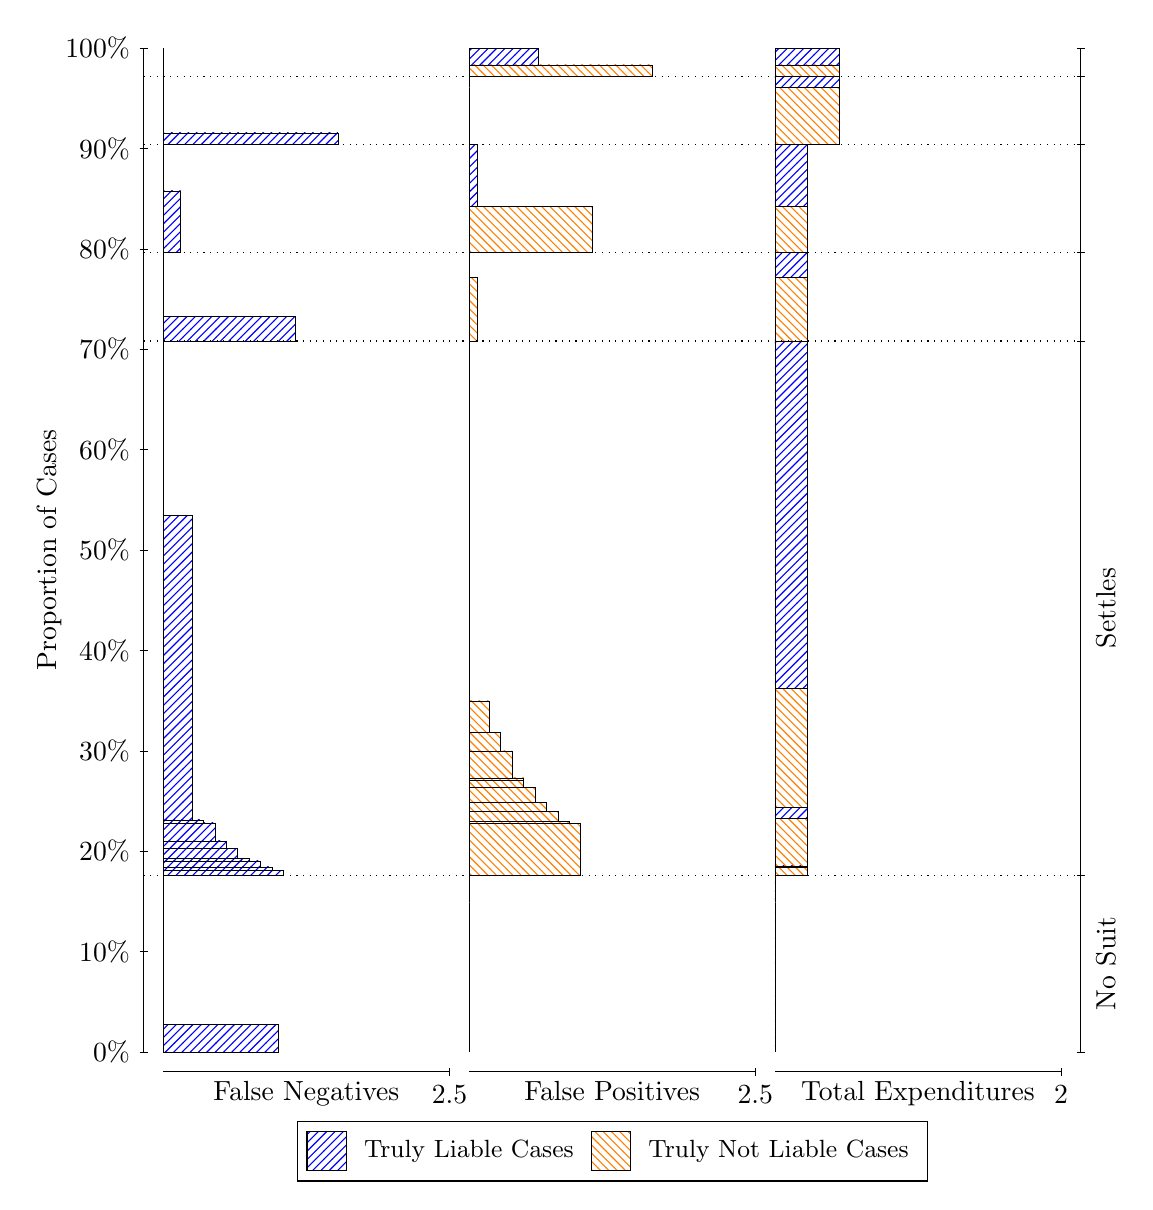
\begin{tikzpicture}
\draw[black, very thin] (1.5,1.75) -- (1.5,14.5);
\node[rotate=90, text=black, anchor=center] at (0.3, 8.125) {Proportion of Cases};
\draw[black, very thin] (1.45,1.75) -- (1.55,1.75);
\node[text=black, anchor=east] at (1.45, 1.75) {0\%};
\draw[black, very thin] (1.45,3.025) -- (1.55,3.025);
\node[text=black, anchor=east] at (1.45, 3.025) {10\%};
\draw[black, very thin] (1.45,4.3) -- (1.55,4.3);
\node[text=black, anchor=east] at (1.45, 4.3) {20\%};
\draw[black, very thin] (1.45,5.575) -- (1.55,5.575);
\node[text=black, anchor=east] at (1.45, 5.575) {30\%};
\draw[black, very thin] (1.45,6.85) -- (1.55,6.85);
\node[text=black, anchor=east] at (1.45, 6.85) {40\%};
\draw[black, very thin] (1.45,8.125) -- (1.55,8.125);
\node[text=black, anchor=east] at (1.45, 8.125) {50\%};
\draw[black, very thin] (1.45,9.4) -- (1.55,9.4);
\node[text=black, anchor=east] at (1.45, 9.4) {60\%};
\draw[black, very thin] (1.45,10.675) -- (1.55,10.675);
\node[text=black, anchor=east] at (1.45, 10.675) {70\%};
\draw[black, very thin] (1.45,11.95) -- (1.55,11.95);
\node[text=black, anchor=east] at (1.45, 11.95) {80\%};
\draw[black, very thin] (1.45,13.225) -- (1.55,13.225);
\node[text=black, anchor=east] at (1.45, 13.225) {90\%};
\draw[black, very thin] (1.45,14.5) -- (1.55,14.5);
\node[text=black, anchor=east] at (1.45, 14.5) {100\%};

\draw[black, very thin] (13.4,1.75) -- (13.4,14.5);
\draw[black, very thin] (13.35,1.75) -- (13.45,1.75);
\node[anchor=west] at (13.35, 1.75) {};
\draw[black, very thin] (13.35,3.995) -- (13.45,3.995);
\node[anchor=west] at (13.35, 3.995) {};
\draw[black, very thin] (13.35,10.779) -- (13.45,10.779);
\node[anchor=west] at (13.35, 10.779) {};
\draw[black, very thin] (13.35,11.9) -- (13.45,11.9);
\node[anchor=west] at (13.35, 11.9) {};
\draw[black, very thin] (13.35,13.275) -- (13.45,13.275);
\node[anchor=west] at (13.35, 13.275) {};
\draw[black, very thin] (13.35,14.144) -- (13.45,14.144);
\node[anchor=west] at (13.35, 14.144) {};
\draw[black, very thin] (13.35,14.5) -- (13.45,14.5);
\node[anchor=west] at (13.35, 14.5) {};

\draw[black, very thin, pattern color=blue, pattern=north east lines] (1.75,1.75) rectangle (3.2033,2.0995);
\draw[black, very thin, pattern color=orange, pattern=north west lines] (1.75,2.0995) rectangle (1.75,3.995);
\draw[black, very thin, pattern color=blue, pattern=north east lines] (1.75,3.995) rectangle (3.276,4.052);
\draw[black, very thin, pattern color=blue, pattern=north east lines] (1.75,4.052) rectangle (3.1307,4.1011);
\draw[black, very thin, pattern color=blue, pattern=north east lines] (1.75,4.1011) rectangle (2.9853,4.1774);
\draw[black, very thin, pattern color=blue, pattern=north east lines] (1.75,4.1774) rectangle (2.84,4.2086);
\draw[black, very thin, pattern color=blue, pattern=north east lines] (1.75,4.2086) rectangle (2.6947,4.3334);
\draw[black, very thin, pattern color=blue, pattern=north east lines] (1.75,4.3334) rectangle (2.5493,4.4309);
\draw[black, very thin, pattern color=blue, pattern=north east lines] (1.75,4.4309) rectangle (2.404,4.6602);
\draw[black, very thin, pattern color=blue, pattern=north east lines] (1.75,4.6602) rectangle (2.2587,4.6986);
\draw[black, very thin, pattern color=blue, pattern=north east lines] (1.75,4.6986) rectangle (2.1133,8.5649);
\draw[black, very thin, pattern color=orange, pattern=north west lines] (1.75,8.5649) rectangle (1.75,10.779);
\draw[black, very thin, pattern color=blue, pattern=north east lines] (1.75,10.779) rectangle (3.4213,11.089);
\draw[black, very thin, pattern color=orange, pattern=north west lines] (1.75,11.089) rectangle (1.75,11.9);
\draw[black, very thin, pattern color=blue, pattern=north east lines] (1.75,11.9) rectangle (1.968,12.687);
\draw[black, very thin, pattern color=orange, pattern=north west lines] (1.75,12.687) rectangle (1.75,13.275);
\draw[black, very thin, pattern color=blue, pattern=north east lines] (1.75,13.275) rectangle (3.9663,13.421);
\draw[black, very thin, pattern color=orange, pattern=north west lines] (1.75,13.421) rectangle (1.75,14.144);
\draw[black, very thin, pattern color=orange, pattern=north west lines] (1.75,14.144) rectangle (1.75,14.286);
\draw[black, very thin, pattern color=blue, pattern=north east lines] (1.75,14.286) rectangle (1.75,14.5);
\draw[black, very thin, pattern color=orange, pattern=north west lines] (5.6333,1.75) rectangle (5.6333,3.6455);
\draw[black, very thin, pattern color=blue, pattern=north east lines] (5.6333,3.6455) rectangle (5.6333,3.995);
\draw[black, very thin, pattern color=orange, pattern=north west lines] (5.6333,3.995) rectangle (7.0503,4.651);
\draw[black, very thin, pattern color=orange, pattern=north west lines] (5.6333,4.651) rectangle (6.905,4.6825);
\draw[black, very thin, pattern color=orange, pattern=north west lines] (5.6333,4.6825) rectangle (6.7597,4.8007);
\draw[black, very thin, pattern color=orange, pattern=north west lines] (5.6333,4.8007) rectangle (6.6143,4.9219);
\draw[black, very thin, pattern color=orange, pattern=north west lines] (5.6333,4.9219) rectangle (6.469,5.1088);
\draw[black, very thin, pattern color=orange, pattern=north west lines] (5.6333,5.1088) rectangle (6.3237,5.2033);
\draw[black, very thin, pattern color=orange, pattern=north west lines] (5.6333,5.2033) rectangle (6.3237,5.2296);
\draw[black, very thin, pattern color=orange, pattern=north west lines] (5.6333,5.2296) rectangle (6.1783,5.5727);
\draw[black, very thin, pattern color=orange, pattern=north west lines] (5.6333,5.5727) rectangle (6.033,5.8091);
\draw[black, very thin, pattern color=orange, pattern=north west lines] (5.6333,5.8091) rectangle (5.8877,6.209);
\draw[black, very thin, pattern color=blue, pattern=north east lines] (5.6333,6.209) rectangle (5.6333,10.779);
\draw[black, very thin, pattern color=orange, pattern=north west lines] (5.6333,10.779) rectangle (5.7423,11.59);
\draw[black, very thin, pattern color=blue, pattern=north east lines] (5.6333,11.59) rectangle (5.6333,11.9);
\draw[black, very thin, pattern color=orange, pattern=north west lines] (5.6333,11.9) rectangle (7.1957,12.489);
\draw[black, very thin, pattern color=blue, pattern=north east lines] (5.6333,12.489) rectangle (5.7423,13.275);
\draw[black, very thin, pattern color=orange, pattern=north west lines] (5.6333,13.275) rectangle (5.6333,13.999);
\draw[black, very thin, pattern color=blue, pattern=north east lines] (5.6333,13.999) rectangle (5.6333,14.144);
\draw[black, very thin, pattern color=orange, pattern=north west lines] (5.6333,14.144) rectangle (7.9587,14.286);
\draw[black, very thin, pattern color=blue, pattern=north east lines] (5.6333,14.286) rectangle (6.5053,14.5);
\draw[black, very thin, pattern color=orange, pattern=north west lines] (9.5167,1.75) rectangle (9.5167,3.6455);
\draw[black, very thin, pattern color=blue, pattern=north east lines] (9.5167,3.6455) rectangle (9.5167,3.995);
\draw[black, very thin, pattern color=orange, pattern=north west lines] (9.5167,3.995) rectangle (9.9254,4.0896);
\draw[black, very thin, pattern color=blue, pattern=north east lines] (9.5167,4.0896) rectangle (9.9254,4.1147);
\draw[black, very thin, pattern color=orange, pattern=north west lines] (9.5167,4.1147) rectangle (9.9254,4.7205);
\draw[black, very thin, pattern color=blue, pattern=north east lines] (9.5167,4.7205) rectangle (9.9254,4.852);
\draw[black, very thin, pattern color=orange, pattern=north west lines] (9.5167,4.852) rectangle (9.9254,6.3657);
\draw[black, very thin, pattern color=blue, pattern=north east lines] (9.5167,6.3657) rectangle (9.9254,10.779);
\draw[black, very thin, pattern color=orange, pattern=north west lines] (9.5167,10.779) rectangle (9.9254,11.59);
\draw[black, very thin, pattern color=blue, pattern=north east lines] (9.5167,11.59) rectangle (9.9254,11.9);
\draw[black, very thin, pattern color=orange, pattern=north west lines] (9.5167,11.9) rectangle (9.9254,12.489);
\draw[black, very thin, pattern color=blue, pattern=north east lines] (9.5167,12.489) rectangle (9.9254,13.275);
\draw[black, very thin, pattern color=orange, pattern=north west lines] (9.5167,13.275) rectangle (10.334,13.999);
\draw[black, very thin, pattern color=blue, pattern=north east lines] (9.5167,13.999) rectangle (10.334,14.144);
\draw[black, very thin, pattern color=orange, pattern=north west lines] (9.5167,14.144) rectangle (10.334,14.286);
\draw[black, very thin, pattern color=blue, pattern=north east lines] (9.5167,14.286) rectangle (10.334,14.5);
\draw[black, dotted] (1.5,3.995) -- (13.4,3.995);
\draw[black, dotted] (1.5,10.779) -- (13.4,10.779);
\draw[black, dotted] (1.5,11.9) -- (13.4,11.9);
\draw[black, dotted] (1.5,13.275) -- (13.4,13.275);
\draw[black, dotted] (1.5,14.144) -- (13.4,14.144);
\draw[black, very thin] (1.75,1.5) -- (5.3833,1.5);
\node[text=black, anchor=north] at (3.5667, 1.5) {False Negatives};
\draw[black, very thin] (5.3833,1.45) -- (5.3833,1.55);
\node[text=black, anchor=north] at (5.3833, 1.45) {2.5};

\draw[black, very thin] (5.6333,1.5) -- (9.2667,1.5);
\node[text=black, anchor=north] at (7.45, 1.5) {False Positives};
\draw[black, very thin] (9.2667,1.45) -- (9.2667,1.55);
\node[text=black, anchor=north] at (9.2667, 1.45) {2.5};

\draw[black, very thin] (9.5167,1.5) -- (13.15,1.5);
\node[text=black, anchor=north] at (11.333, 1.5) {Total Expenditures};
\draw[black, very thin] (13.15,1.45) -- (13.15,1.55);
\node[text=black, anchor=north] at (13.15, 1.45) {2};

\node[text=black, centered, rotate=90] at (13.72, 2.8725) {No Suit};
\node[text=black, centered, rotate=90] at (13.72, 7.387) {Settles};





\draw (7.449999999999999,1.5) node[draw=none] (baseCoordinate) {};
\begin{scope}[align=center]
        \matrix[scale=0.5, draw=black, below=0.5cm of baseCoordinate, nodes={draw}, column sep=0.1cm]{
            \node[rectangle, draw, minimum width=0.5cm, minimum height=0.5cm, pattern color=blue, pattern=north east lines] {}; &
            \node[draw=none, font=\small, text=black] (B) {Truly Liable Cases}; &
            \node[rectangle, draw, minimum width=0.5cm, minimum height=0.5cm, pattern color=orange, pattern=north west lines] {}; &
            \node[draw=none, font=\small, text=black] (B) {Truly Not Liable Cases}; \\
            };
\end{scope}

\end{tikzpicture}
\end{document}